	\chapter{Kravspecifikation}
	
	\section{Aktør kontekst diagram}
		På figur \ref{fig:AktorKontekst} ses aktør kontekst diagrammet for Rambøll Tilsyn. Diagrammet viser, hvilke aktør der interagerer med systemet.
	\begin{figure}[H]
		\centering
		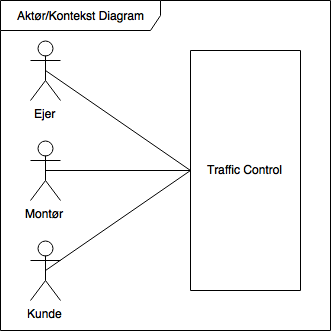
\includegraphics[width=0.6\linewidth]{Kravspecifikation/AktorDiagram}
		\caption{Aktør kontekst diagram for Rambøll Tilsyn}
		\label{fig:AktorKontekst}
	\end{figure}

	På venstre side af figur \ref{fig:AktorKontekst} ses brugeren som er den primære aktør af systemet. Brugeren benytter systemet, som på diagrammet bliver symboliseret som en blackbox. På højre side, ses de sekundære aktører. Disse aktører er dem som systemet bruger. Microsoft Office er en sekundær bruger, da systemet eksportere til Excel.
	
	\clearpage
	
\section{User stories diagram}
	Figur \ref{fig:Userstoriediagram} vises systemets User Stories diagram. Dette diagram viser den funktionalitet som systemet indeholder beskrevet gennem en række user stories.
	
	\begin{figure}[H]
		\centering
		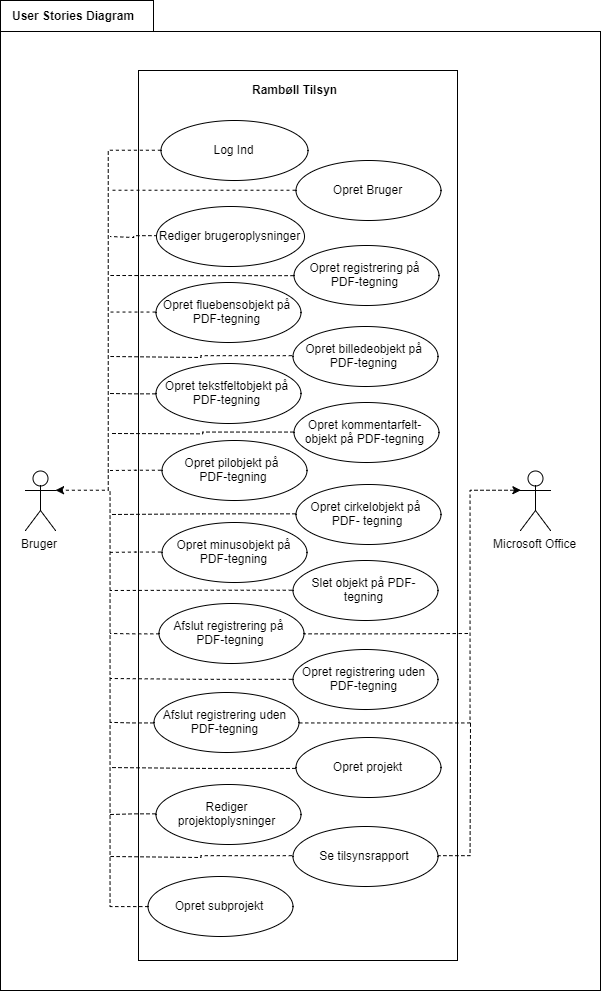
\includegraphics[width=0.6\linewidth]{Kravspecifikation/UserStorieDiagram}
		\caption{User stories diagram for Rambøll Tilsyn}
		\label{fig:Userstoriediagram}
	\end{figure}
	
	\clearpage
	
\section{Funktionelle krav} 
	Følgende er en kort beskrivelse af nogle udvalgte user stories til Rambøll Tilsyn, som er fundet sammen med Rambøll ved hjælp af MoSCoW analyse. \cite{MoSCoW} For alle user stories fuldt beskrevet med Gherkin, se kravspecifikationen afsnit \ref{Krav-sec:UserStories}.

	\subsection*{Log-in (CRS-1)}
	Denne user story håndtere log-in på applikationen. Her skal bruger indtaste korrekt brugernavn og kodeord, for at få adgang.
	
	\subsection*{Opret bruger (CRS-2)}
	Opret bruger user storien giver en bruger mulighed for at oprette en ny bruger til systemet. Når brugeren er blevet oprettet, vil han/hun kunne logge ind på applikationen og benytte systemet.
	
	\subsection*{Opret en registrering på PDF tegning (CRS-4)}
	Denne user story håndtere det at brugeren ønsker at oprette en registrering til et byggeprojekt, hvor at bruger har en PDF tegning at registre på. 
	
	\subsection*{Opret fluebens objekt på PDF tegning (CRS-5)}
	I denne user story får brugeren mulighed for at sætte et flueben på PDF tegningen i sin registrering. Denne bruges af brugeren til at vise om denne del af byggeriet er godkendt.

	\subsection*{Opret billede objekt på PDF tegning (CRS-6)}
	Denne user story giver brugeren mulighed for at tage et billede og placere på PDF tegningen. Når billedet er taget og placeret på PDF'en kan bruger skrive en kort beskrivende tekst til billedet.
		
	\subsection*{Slet objekt på PDF tegning (CRS-12)}
	I denne user story for bruger mulighed for at slette et objekt. Hvis bruger placere et objekt forkert, eller kommer til at vælge det forkerte objekt, kan bruger slette objektet. 

	\subsection*{Afslut registrering på PDF tegning (CRS-13)}
	Denne user story håndtere afslutningen af brugeren registrering. Når brugeren har oprettet alle sine objekter på PDF'en, kan der vælges afslut og en excel fil vil blive genereret med information om de forskellige objekter.
	
	\subsection*{Opret projekt (CRS-16)}
	Opret projekt user storien giver bruger mulighed for at oprette nye projekter i systemet. Når projektet er oprettet ville brugere kunne tilgå dette projekt og oprette registreringer. \\
	

\section{Ikke-funktionelle krav}
De ikke-funktionelle krav definere de tekniske krav som systemet skal indeholde. Disse krav beskriver egenskaber som ikke har indvirkning på systemets funktionelle krav. Dette kunne være antal brugere der benytter systemet samtidig eller hvordan brugerne skal have skrive og læse rettigheder. \\
Projektes ikke-funktionelle krav kan findes i afsnit \ref{Krav-sec:Ikkefunktionelle} i kravspecifikationen under bilag. \\


\section{Afgrænsning}
For at afgrænse projektet blev der holdt et møde med Rambøll, hvor de kunne komme med inputs til systemet. \\
Der blev lavet en MoSCoW analyse til at prioriterer funktionaliteten i systemet. Denne analyse form deler alt funktionaliteten op i fire kategorier \emph{must}, \emph{should}, \emph{could} og \emph{would}.
Det blev valgt at systemets \emph{must} user stories definere systemet og derved at disse funktionaliteter som er blevet implementeret i projektet. \\
Rambøll ønskede en applikation udviklet med fokus på iOS, da største delen af afdelingen har iPads tilknyttet. Der var dog en længere snak omkring dette, da også et par enkelte brugte Android. Derfor blev det aftalt at der ville forsøges med at udvikle i cross-platform, som ville kunne fungere til både iOS og Android. Men hvis det blev tidspresset skulle fokus ligge på at udvikle til iOS. \\
For den fulde afgrænsning samt MoSCoW analyse, henvises til kravspecifikationens afsnit \ref{Krav-sec:Afgraensning}.
	